\section{System Overview}
Through the system overview diagram, in figure \ref{fig:system_overview}, it is possible to identify the main modules of the system to be developed, and how they interact. We can divide the system into three subsystems: the local system, which represents a lamppost, the gateway, a device that links the lampposts network to the remote server, and the remote system, that stores information about the lamppost network and allows interaction with the system users by the use of remote client applications.

\begin{figure}[H]
	\centering
	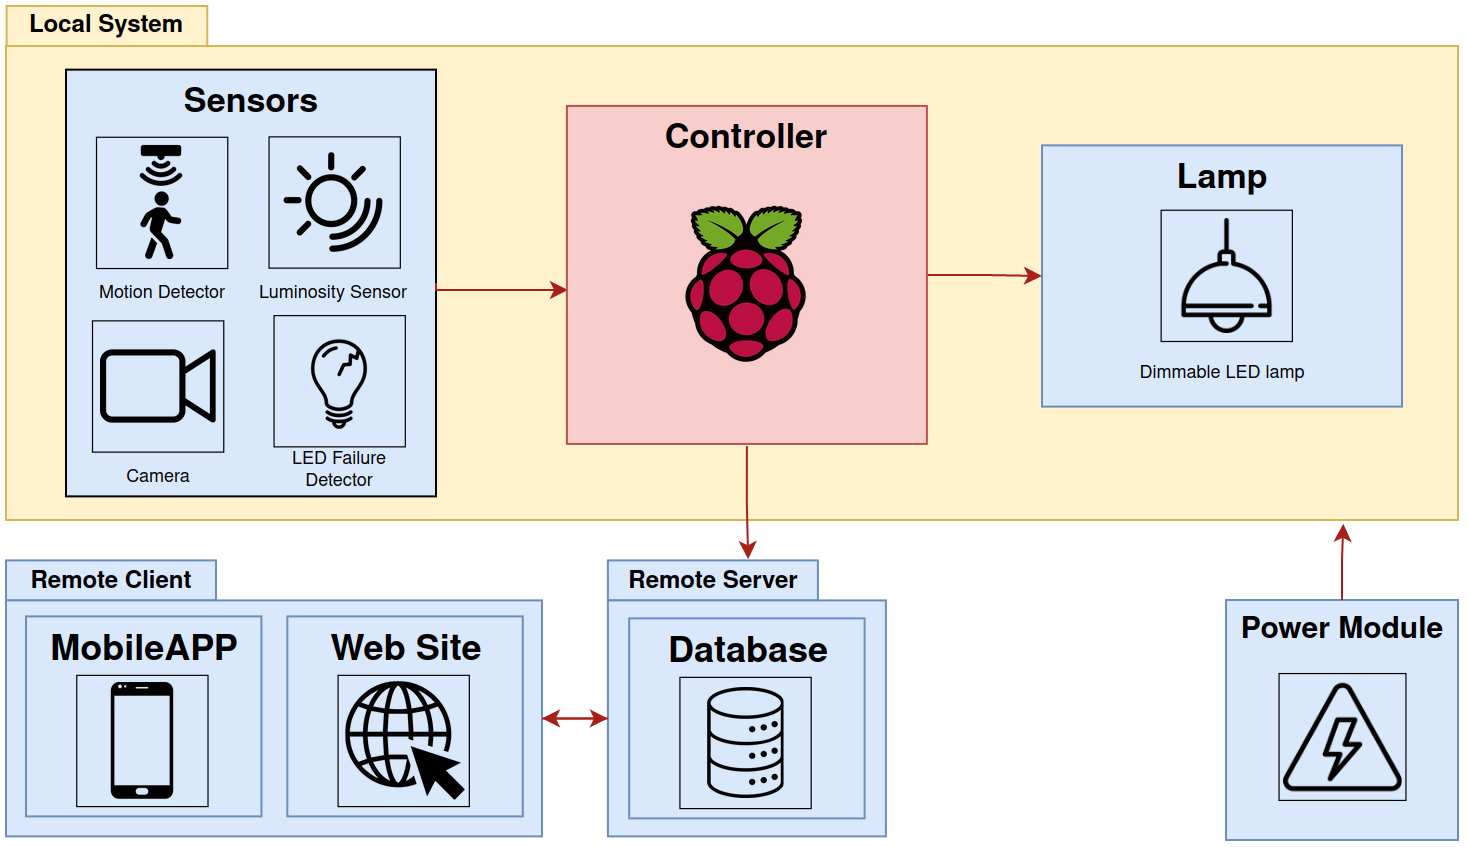
\includegraphics[width=0.95\textwidth]{03system_overview/system_overview}
	\caption{System Overview Diagram.}
	\label{fig:system_overview}
\end{figure}

The local system is composed of sensors, a controller, a lamp and a wireless communication module, LoRa module. Regarding the sensors, there will be a motion detector, to allow the detection of movement in the vicinity of the pole, a luminosity sensor, to detect the light conditions of the pole’s surroundings, a lamp failure detector to know if the lamp is working and a camera to detect empty parking spots in the lamppost vicinity. The controller of the local system is a Raspberry Pi, that uses the sensors information and communicates wirelessly with the gateway using a LoRa communication module. The gateway also communicates through internet with a remote server, so that network information is stored in the remote server, and to allow the dynamic control of local systems.

The remote system is composed by the remote server and the remote client. The remote server consists of a database that stores all information about each lamppost location and operating status. This information can be accessed through a mobile application by the operator in order to carry out the necessary maintenance of the lamp of each pole. Furthermore, the operator, when installing a new lamppost, can add its location to the database, using the mobile application. In addition, the database stores information on available parking spaces detected by the camera. When a user, a car driver, wants to know where there are empty parking places, he can access a website that informs him of the location of the empty parking spaces.

%Knowing that the public lighting network is directly related to the electrical network, this will be used to power each local system.

\section{System Architecture}
Using the system overview diagram information, one can describe the system in two different architectures: hardware architecture, as how the hardware modules interfaces with itself, what are the physical components of the system, and software architecture, which details how the information is processed among different software layers.

\clearpage
\subsection{Hardware Architecture}

\subsubsection{Local System}

In figure \ref{fig:local_hw_arch}, one can see the diagram that represents the main hardware components of the system.

The Raspberry Pi is the main component in the system, processing all the information given by the sensors and the camera. The Raspberry Pi is connected to a LoRa module, for the local system communicate with the remote system. In order to control the lamp brightness, a driver is used, taking a signal from the Raspberry Pi, and system power as inputs.

The local system is powered by the power grid, through a power module. This module contains an \ac{ac}/\ac{dc} converter, and eventually a step-down converter, to power the Raspberry Pi and its associated sensors.

\begin{figure}[ht]
	\centering
	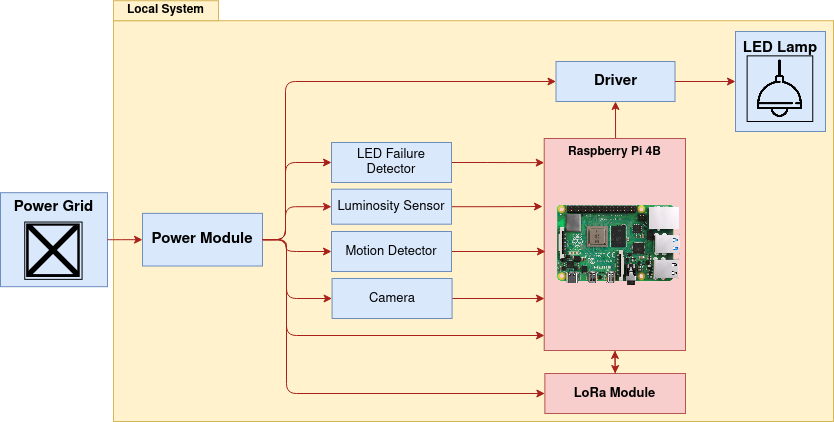
\includegraphics[width=1\textwidth]{03system_overview/local_hw_arch}
	\caption{Local System Hardware Architecture Diagram.}
	\label{fig:local_hw_arch}
\end{figure}

\clearpage
\subsubsection{Gateway}

The hardware architecture of the gateway is shown in figure \ref{fig:gateway_hw_arch}. The purpose of this device is to  link the local systems to the remote system, so the hardware needed is only the LoRa communication module, as well as the Raspberry Pi to manage all communications.

As in the local system, there is a power module to power the gateway components, the Raspberry Pi and LoRa module.

%\clearpage 
\begin{figure}[H]
	\centering
	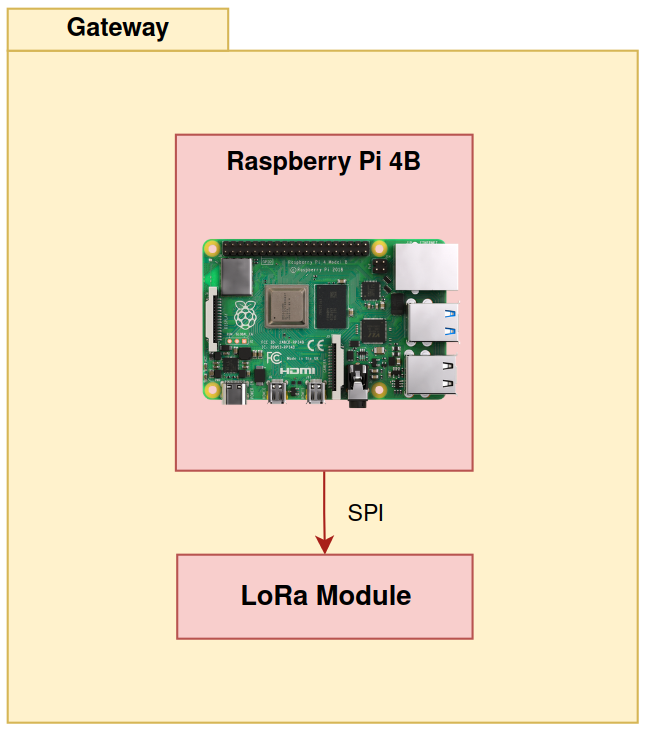
\includegraphics[width=0.85\textwidth]{03system_overview/gateway_hw_arch}
	\caption{Gateway Hardware Architecture Diagram.}
	\label{fig:gateway_hw_arch}
\end{figure}

\subsection{Software Architecture}
The software architecture is divided into three layers:
\begin{itemize}
        \item The \textbf{Operating System} layer, which is composed by the Operating System drivers and Board Support Packages;
        \item The \textbf{Middleware} layer, which includes software for abstracting the lower level layer packages. It works as a pipe since it links two applications, in different layers, so that data can be easily transmitted;
        \item The \textbf{Application} layer, where the core functionality of the program is built, with a resource for the API's in the lower level layers.
\end{itemize}

\clearpage
\subsubsection{Local System}

As shown in figure \ref{fig:local_sw_arch}, the operating system layer is composed by the sensor drivers, such as the LED Failure Sensor, the Luminosity Sensor, the Motion Detector, the camera, and also the LoRa communication driver. In the middleware layer are the tools needed to process the images from the camera, to acquire data from sensors and to communicate via LoRa protocol with the gateway. The application layer manages the communication with the gateway.

\begin{figure}[H]
	\centering
	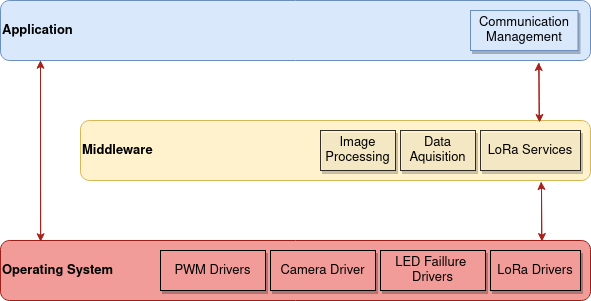
\includegraphics[width=.85\textwidth]{03system_overview/local_sw_arch}
	\caption{Local System Software Architecture Diagram.}
	\label{fig:local_sw_arch}
\end{figure}

\clearpage
\subsubsection{Gateway}
In figure \ref{fig:gateway_sw_arch} is shown the software architecture of the gateway device. The operating system layer is composed by the communication drivers, responsible of providing resources to establish a TCP/IP connection, with the remote system, and establish a LoRa connection with the local systems. The middleware layer deals with LoRa services and with TCP/IP framework. The application layer manages all communications between the street lampposts network and the remote system.

\begin{figure}[H]
	\centering
	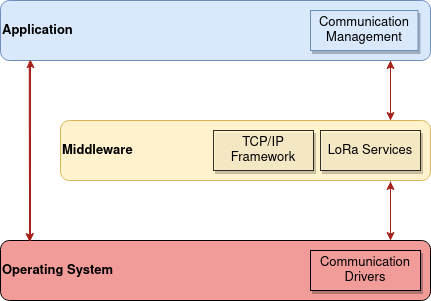
\includegraphics[width=.75\textwidth]{03system_overview/gateway_sw_arch}
	\caption{Gateway Software Architecture Diagram.}
	\label{fig:gateway_sw_arch}
\end{figure}

\clearpage
\subsubsection{Remote System}
In figure \ref{fig:remote_sw_arch} is shown the software architecture of the remote system. The operating system layer is composed by the communication drivers, more specifically, TCP/IP, that are needed to establish a connection with the gateway. In the middleware layer, there is the TCP/IP framework.
In the application layer there is the \ac{gui}, that allows the interaction with the user, through a mobile application and a web site. There are also the communication and database management, responsible of editing the database when required and supplying all the information requested by the \ac{gui}.

\begin{figure}[H]
	\centering
	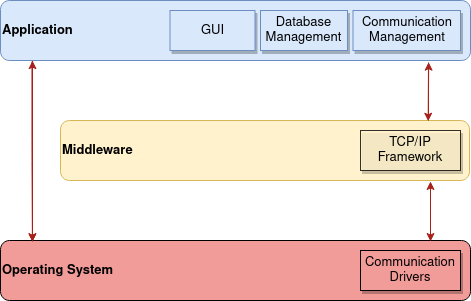
\includegraphics[width=.75\textwidth]{03system_overview/remote_sw_arch}
	\caption{Remote System Software Architecture Diagram.}
	\label{fig:remote_sw_arch}
\end{figure}

\clearpage
\subsection{Database E-R Diagram}
In the database will be stored all the information about each lamppost, its operators and parking spots. In the figure \ref{fig:Database} one can see the Entity Relationship Diagram (E-R Diagram), displaying the relationships between the entities.

This database has five entities: "Lamppost", "Location", "Region", "Operator" and "Parking Space". A lamppost has a unique identification, his location coordinates and the status of the lamp (lamp at minimum bright level/ lamp at maximum bright level/ lamp OFF/ lamp broken). The location is defined by the coordinates, the post code associated and the street name. A region has multiple locations associated, that are defined by the post code. This entity has also information about parish, county, district of the specified region and the operator responsible for the lampposts in that region. The entity "operator" has the operator identification, the operator name and the operator pin code (used to login in the mobile application). A parking spot is defined by the entity "Parking Space" and has the attributes identification of the parking space, its location coordinates, the parking space type (normal park/ park for disabled people/ restrict park) and the park status (available/ not available).

%\subsubsection{Relational Model}
%
%lamppost(\uline{pole\_id}, \dotuline{gps}, pole\_status)
%
%location(\uline{gps}, \dotuline{post\_code}, street\_name)
%
%region(\uline{post\_code}, \dotuline{operator\_id}, parish, county, district)
%
%operator(\uline{operator\_id}, operator\_name)
%
%parking\_space(\uline{park\_id}, \dotuline{gps}, park\_type, park\_status)

\begin{figure}[ht]
        \centering
        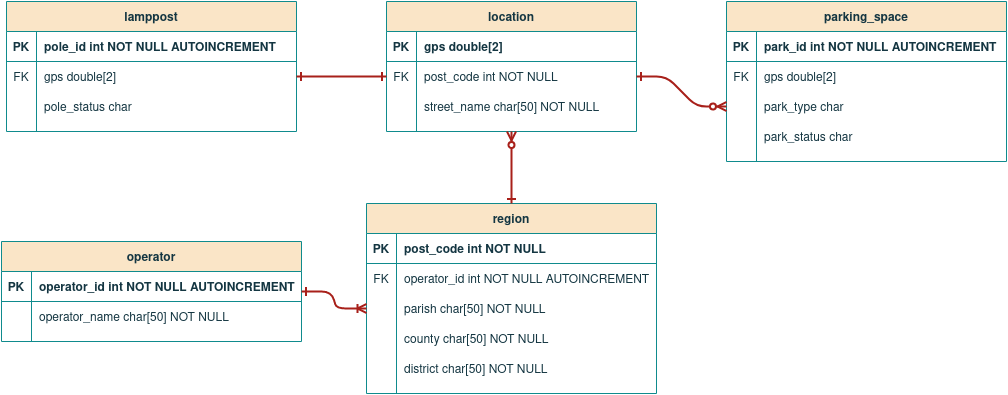
\includegraphics[width=1\textwidth]{03system_overview/database}
        \caption{Database E-R Diagram.}
        \label{fig:Database}
\end{figure}

